% Chris's Entropy Library - User Guide - Quadratic Extrapolation
% Written by Christopher Thomas.

\chapter{Quadratic Extrapolation}
\label{sect-extrap}

This library's calculations of conditional entropy, mutual information,
and transfer entropy are estimates. These estimates converge on the true
values as the number of samples is increased. A rigorous analysis of the
effect of small sample sizes on estimates typically performed with neural
data is presented in Treves 1995. The take-away from that work is that
entropy tends to be over-estimated, and that the estimate tends to converge
monotonically on the correct value as sample size is increased. An example
of this convergence for mutual information estimated using this library is
shown in Figure \ref{fig-extrap-mi} (left pane).

A follow-up analysis presented in Strong 1998 showed that for sample counts
above a threshold, the true entropy value could be estimated by
curve-fitting estimates from finite sample counts and extrapolating the
curve fit to infinite sample counts. An example of applying this
extrapolation method to mutual information estimation using this library is
shown in Figure \ref{fig-extrap-mi} (right pane). Note that the estimate
converges more quickly but is no longer monotonic.

\figdef{\begin{tabular}{ccc}
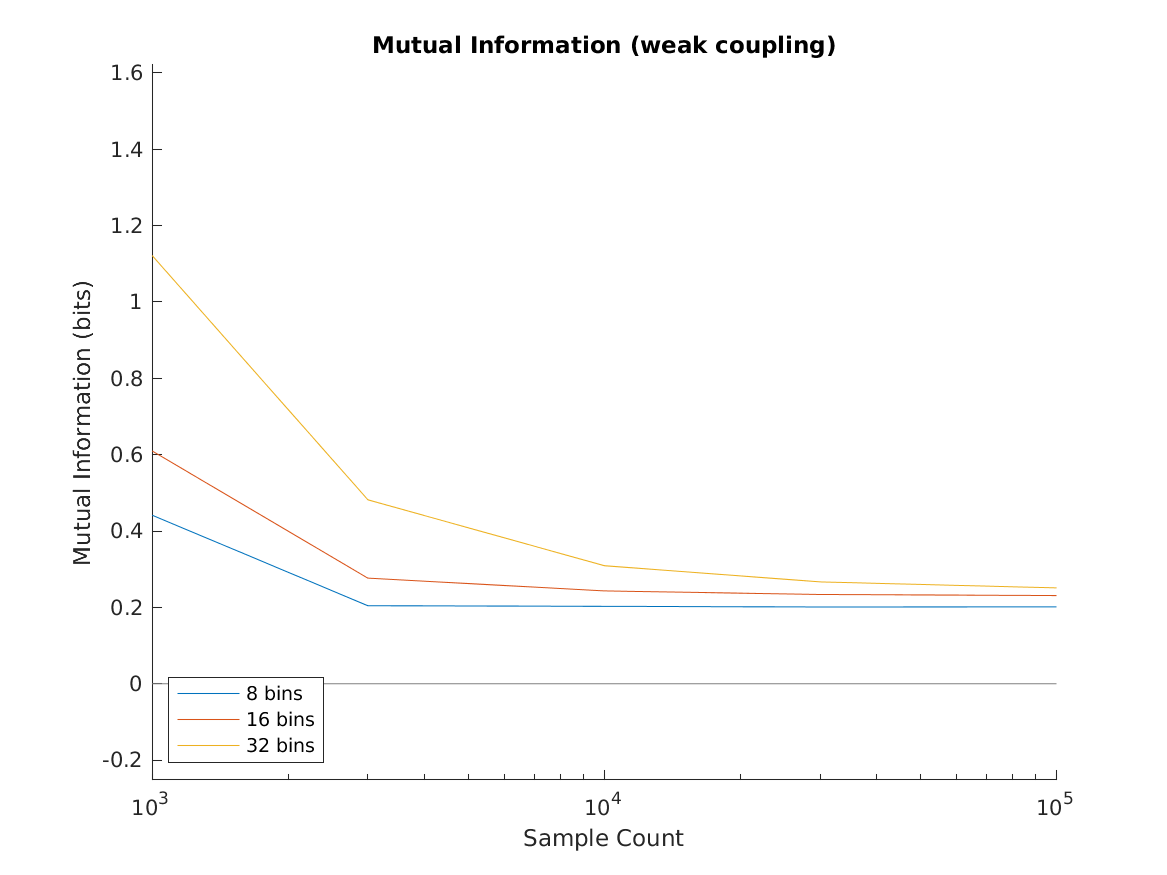
\includegraphics[width=0.45\textwidth]{plots/mutual-weak-raw.png} & ~ &
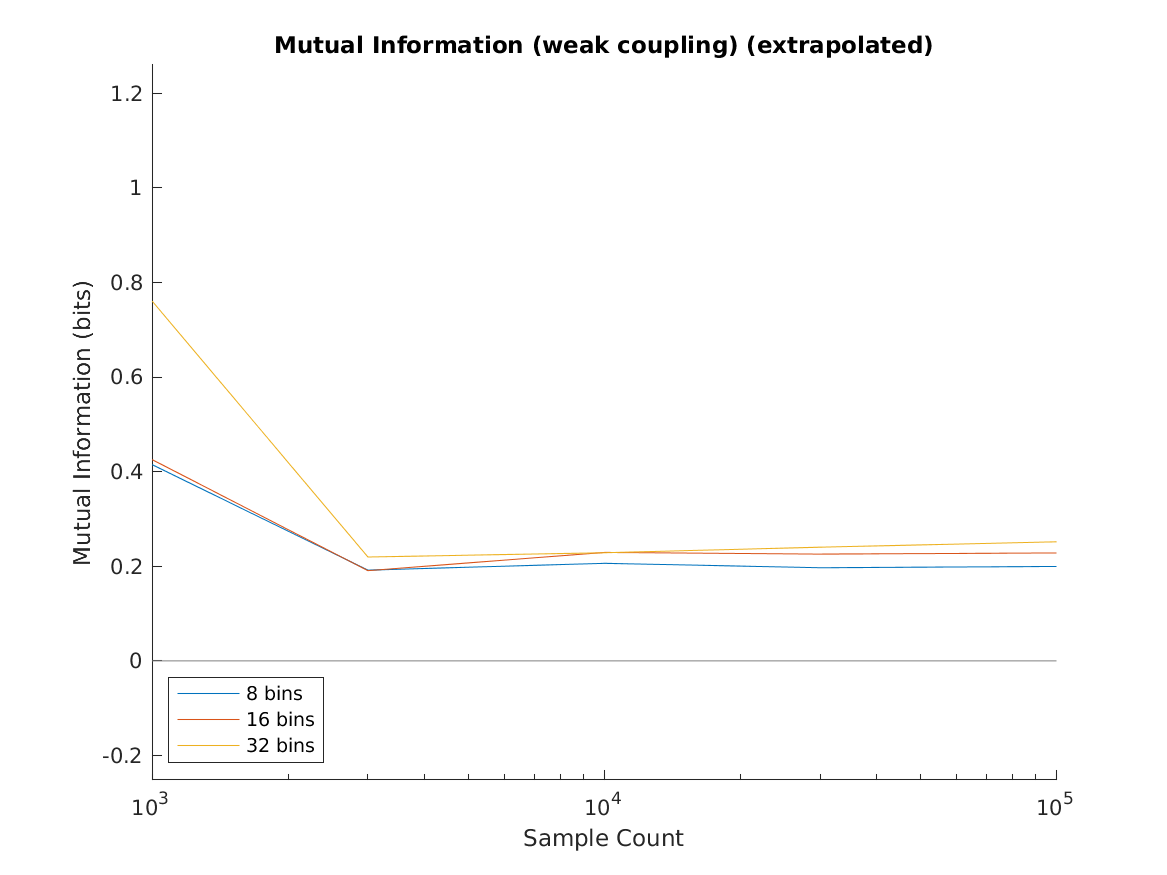
\includegraphics[width=0.45\textwidth]{plots/mutual-weak-extrap} \\
\end{tabular}}
{Mutual information between weakly coupled signals computed without
extrapolation (left) and with extrapolation (right), as a function of the
number of samples used to produce the estimate.}
{fig-extrap-mi}

This library's implementation of the extrapolation algorithm is based on
description given in Palmigiano 2017, used in that work for the estimation
of transfer entropy. In this library it may be used (at the user's
discretion) for the estimation of conditional entropy, mutual information,
and transfer entropy.

The algorithm is supplied with several divisor values $N_{div}$. For each
divisor value several random subsets of the data of size $N_{samp}
\div N_{div}$ are chosen. The metric to be estimated is evaluated for each
of these random subsets, and the results are averaged to produce an estimate
associated with that $N_{div}$. A quadratic curve fit is performed as a
function of $N_{div}$. This is used to estimate the metric value at
$N_{div} = 0$, which corresponds to an infinite number of samples.

As noted in Strong 1998, there is a minimum sample count below which this
estimation method fails. With or without quadratic extrapolation, it will
be necessary to test several sample counts to evaluate whether the estimate
has converged or not. In testing, the practical impact of extrapolation was
to reduce the number of samples needed for convergence by approximately
$3\times$ to $10\times$.

\section{References}
\label{sect-extrap-refs}

\begin{itemize}
%
\item A. Treves, S. Panzeri, \textit{The Upward Bias in Measures of
Information Derived from Limited Data Samples}, Neural computation,
v~7, pp~399-407, 1995
%
\item S. P. Strong, R. Koberle, R. R. de Ruyter van Steveninck, W. Bialek,
\textit{Entropy and Information in Neural Spike Trains},
Physical Review Letters, v~80, no.~1, pp~197-200, January 1998
%
\item A. Palmigiano, T. Geisel, F. Wolf, D. Battaglia,
\textit{Flexible Information Routing by Transient Synchrony},
Nature Neuroscience, v~20, no.~7, pp~1014-1022, 2017
%
\end{itemize}

%
% This is the end of the file.
